%Preámbulo:  
\documentclass{article} %O cualquier otra clase.  
\usepackage[T1]{fontenc}  
\usepackage[utf8]{inputenc}  
\usepackage[english]{babel}  
\usepackage{amsmath,amssymb}
\usepackage[export]{adjustbox}
\usepackage[affil-it]{authblk}
\usepackage[center]{caption}
\usepackage{hyperref}
\hypersetup{
    colorlinks=true,
    linkcolor=black,      
    pdftitle={Nuclear Physics - Computer Lab 2},
    }
\usepackage{graphicx}
\graphicspath{ {C:/Users/luisf/OneDrive - UNIVERSIDAD ALICANTE/UA/Física/Cuarto/1º Cuatrimestre/Física nuclear y de partículas/Práctica 2/Images} }
\author{Luis Lucas García}
\title{Answers to the analysis questions proposed for exercise 2}
\date{\today}
\affil{Facultad de ciencias - Universidad de Alicante - Física nuclear y de partículas - Grupo L3 - Grado en física}
%Documento
\begin{document}
\maketitle
\begin{abstract}
In this document we will answer the questions proposed in the script for exercise 1ç2 of the nuclear physics computer lab. We will analyze the decay of uranium and some chains and compare them with exercise 1 and their binding energies.
\end{abstract}
\tableofcontents

\section{Decay of Uranium}

Firstly, let's plot the analytical solutions for the activity and the remaininc nuclei of the two isotopes of uranium that we are going to study.

\begin{figure}[h!]
\begin{center}
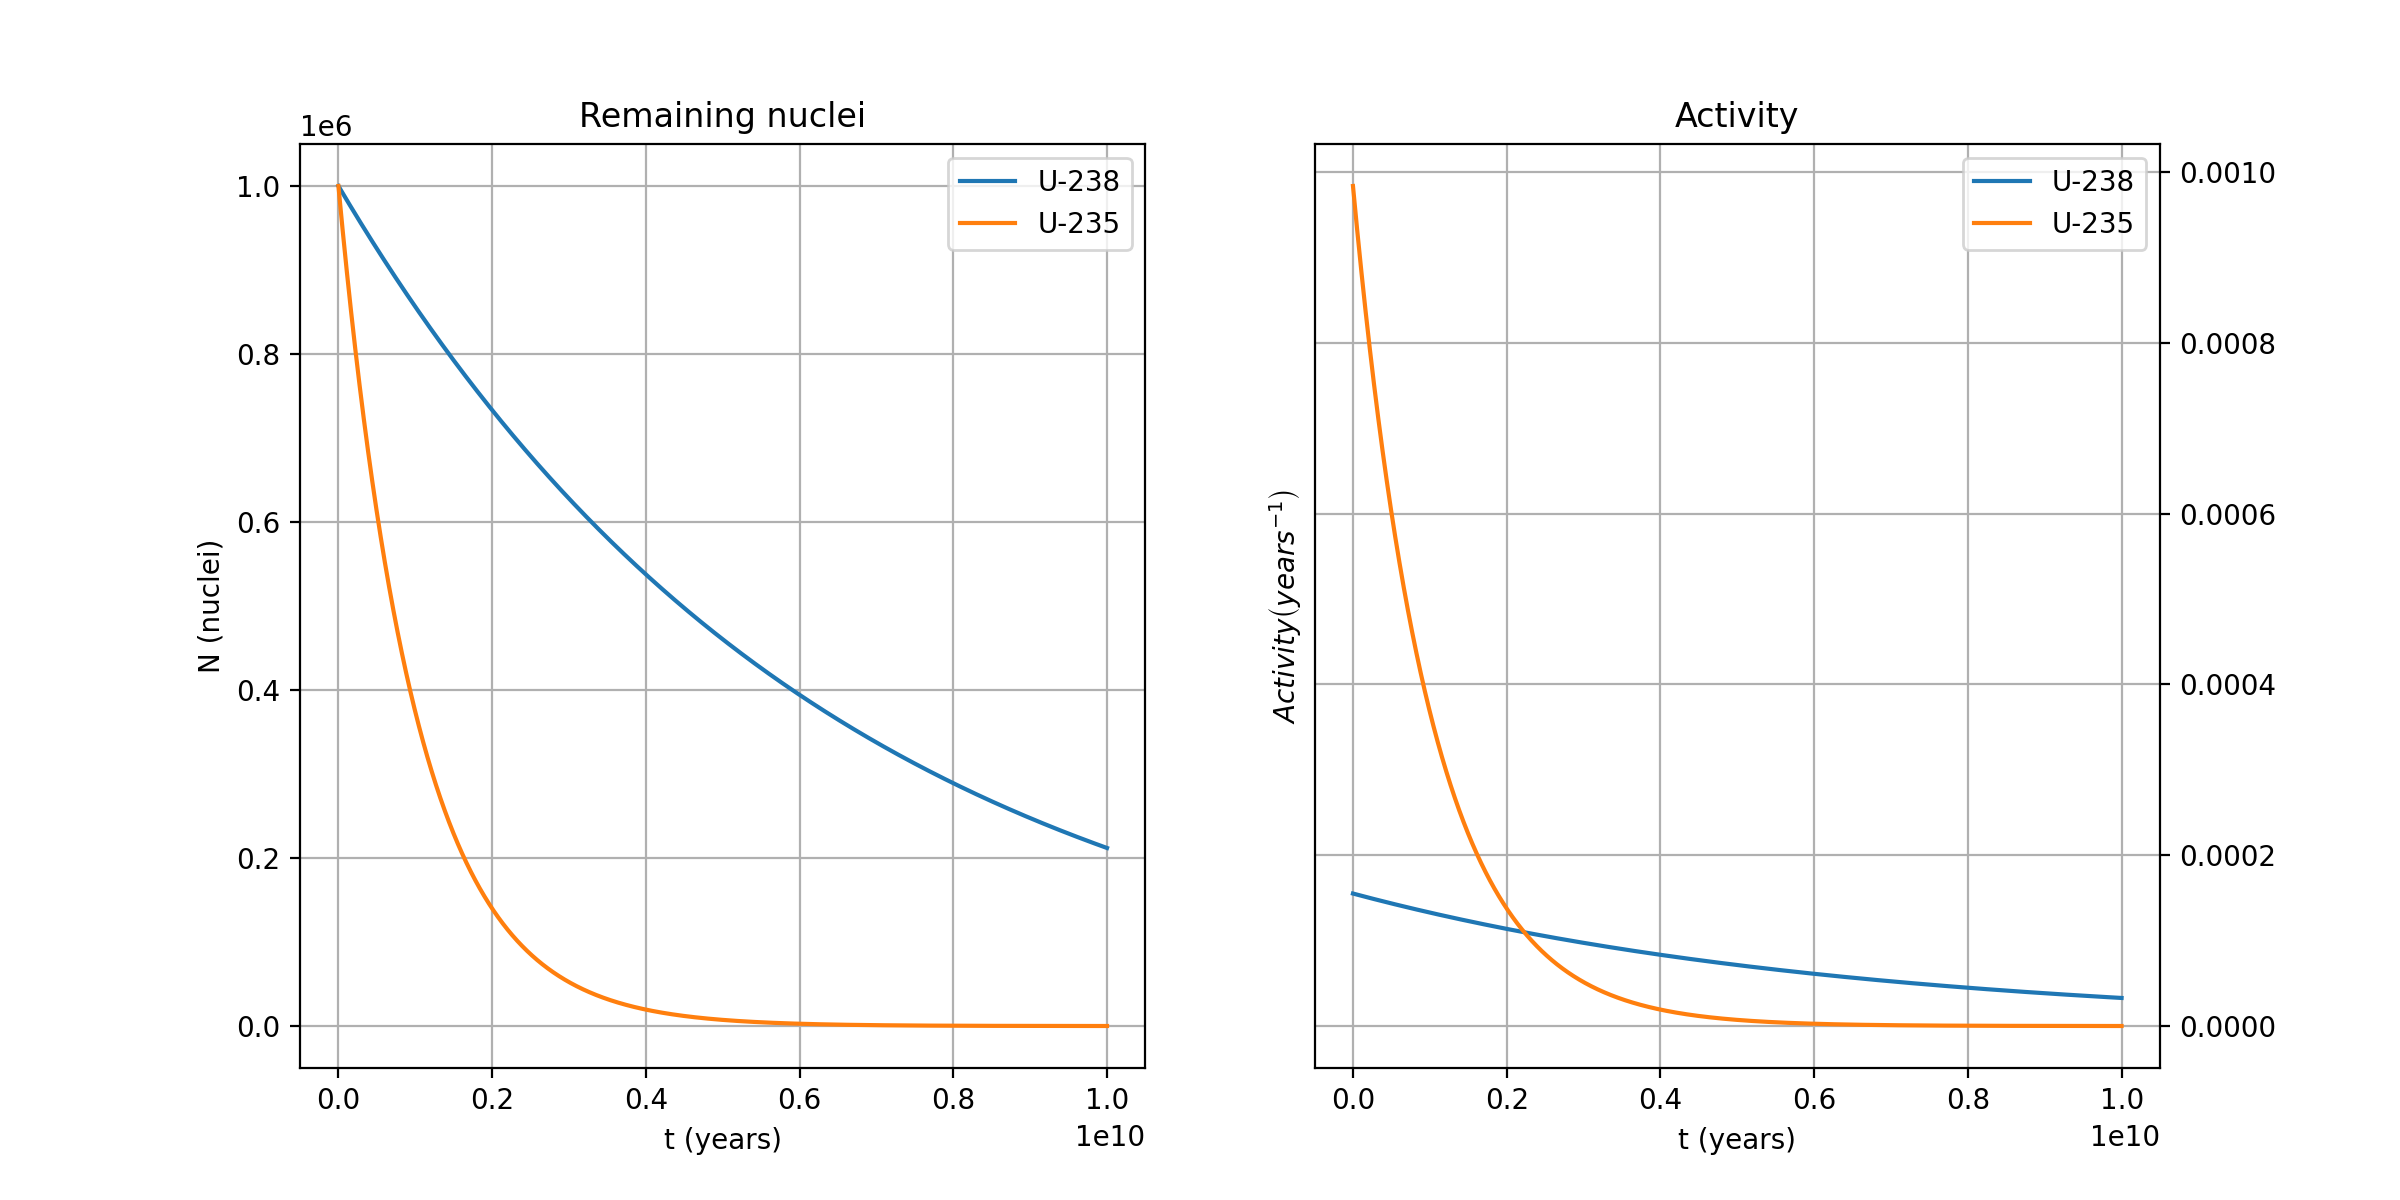
\includegraphics[max width=\linewidth]{Nuclei and activity}
\caption{Nuclei and activity decay for two isotopes of uranium.}
\end{center}
\end{figure}

We can see a very quick drop in nuclei for uranium-235, as well as in activity. This is because it has a shorter lifetime than uranium-238, which makes it more likely for an atom to decay.

More desintegrations mean more activity, which is why for 235 the activity is very high at the beggining but decays so quickly, because atoms disappear faster.

\section{Decay chains}

For this next section we will implement the decay of thorium as well. When uranium decays it generates an isotope of thorium. The amount of this second isotope is given by:

\begin{equation}
N_2(t) = N_1(0)\frac{\lambda_1}{\lambda_2 - \lambda_1} \left( e^{-\lambda_1 t} - e^{-\lambda_2 t} \right)
\end{equation}

With this, we can plot the activity and amount of the both thorium isotopes as well as the uranium ones, with dependence in time.

\begin{figure}[h!]
\begin{center}
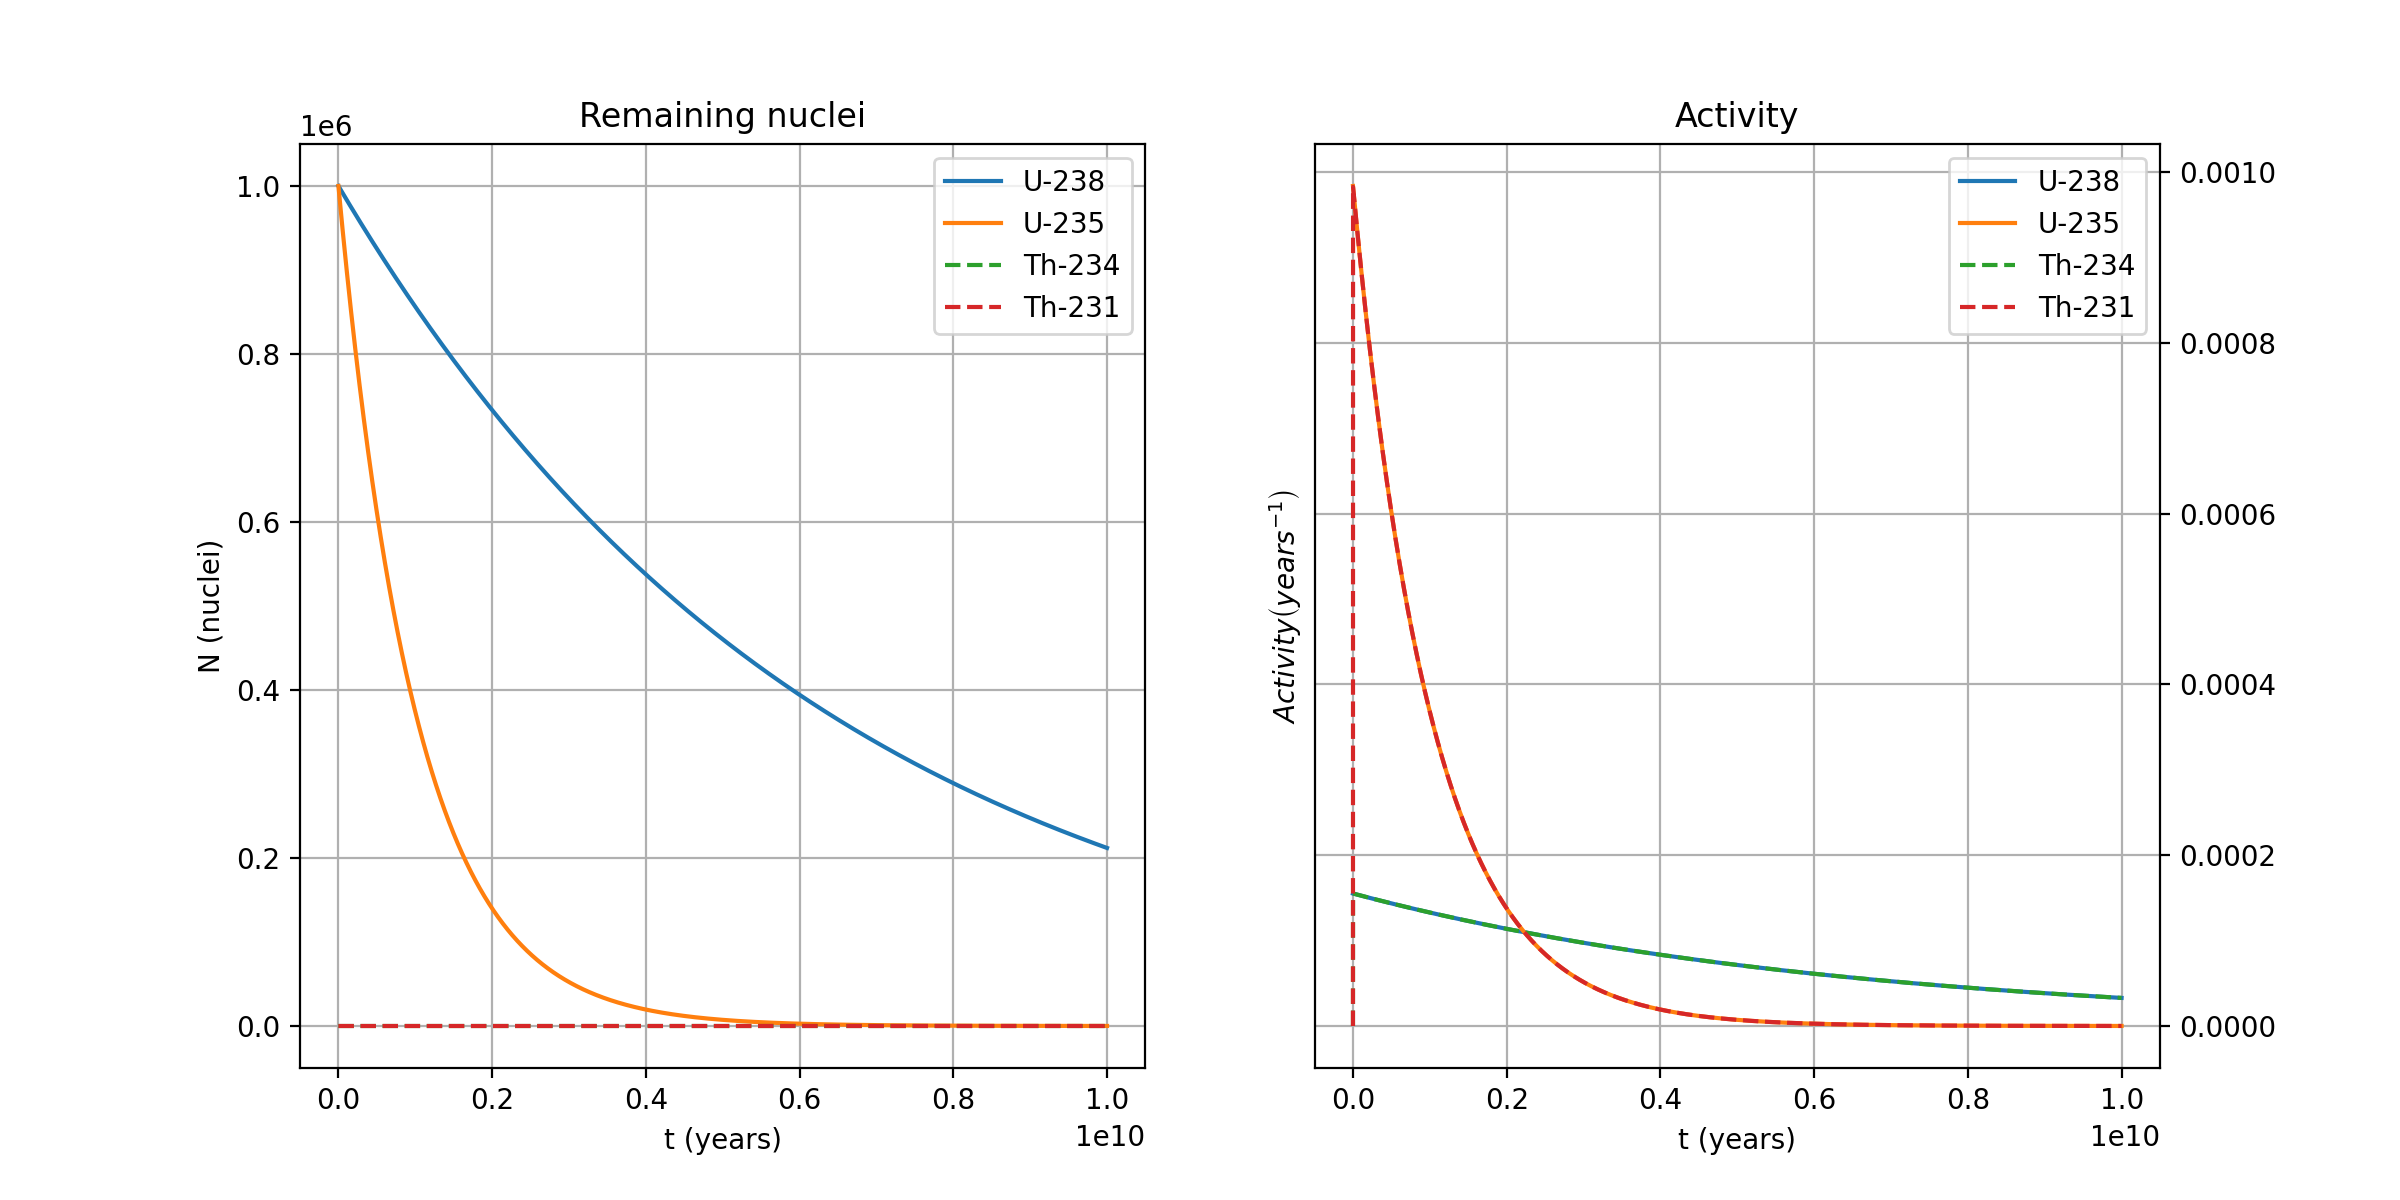
\includegraphics[max width=\linewidth]{Nuclei and activity in chains}
\caption{Amount and activity of the uranium and thorium isotopes.}
\end{center}
\end{figure}

It can be seen that the activity of the product nuclei is almost the same as that of the original nuclei. This is because the products decay much faster than the reactants, so, whenever a daughter nuclei is formed, it is deintegrated very quickly which means there's never a significant amount of nuclei, which means that the activity given by the decay of the products is never significant.

If we calculate the time to obtain a given percentage of the initial concentration we would end up with the next formula:

\begin{equation}
t = -\frac{ln(\alpha)}{\lambda}
\end{equation}

Where $\alpha$ is the percentage. We can build a table with the times for the concetrations asked in the script.

\begin{center}
\begin{tabular}{|c|c|c|}
\hline
Time (Years) & U-238 & U-235 \\ \hline \hline
90\% & $6.79 \times 10^8$ & $1.07 \times 10^8$ \\
50\% & $4.47 \times 10^9$ & $7.05 \times 10^8$ \\
10\% & $1.48 \times 10^{10}$ & $2.34 \times 10^9$ \\ \hline
\end{tabular}
\captionof{table}{Table of the times necessary to reach given amounts of the inicial concentration in the uranium isotopes}
\end{center}

\section{Discussion}

Now, if we compare with the previous exercise, we will find that U-235 was a more stable isotope given its binding energy, however, we have seen that it deintegrates much faster than U-238 since it has a shorter half-life, this seems to be a contradiction with the binding energy.

This difference is explained by the kind of decay that these different isotopes undergo. Uranium-235 goes through an alpha decay which happens more often and can trigger the same decay in close nuclei thanks to the release of neutrons, while uranium-238 undergoes a beta decay, less likely, and doesn't give neutrons, becoming plutonium-239 in its final stage, in a way, uranium-238 acts as an absorber of neutrons.

\section{Uranium-lead dating}

The chain of uranium ends in lead, Pb, which means that we can use it for dating. If we assume that the concentration of lead comes only from uranium, we will have that the atoms of uranium at a given time are:

$$
N_{U} = N_0 e^{-\lambda t}
$$

Where t is the age that we want to evaluate. The initial concentration of uranium is the quantity of lead atoms plus the uranium atoms at a given time, which let us solve for t:

\begin{align*}
U = (Pb + U)e^{-\lambda t} \implies \left( e^{-\lambda t} - 1 \right) U + Pb e^{-\lambda t} = 0 \implies \\ \left( 1 - e^{\lambda t} \right) U + Pb = 0 \implies
\end{align*}
\begin{equation}
\frac{Pb}{U} = e^{\lambda t} - 1
\label{eq:leadDating}
\end{equation}

Since we can know the concentrations of each isotope this lets us know the age of the rock:

\begin{equation}
t = \frac{1}{\lambda} ln \left( \frac{Pb}{U} + 1 \right)
\end{equation}

The equation (\ref{eq:leadDating}) can lead to a linear fit in which the time can appear as the slope. For times in which $\lambda t \approx 0$ then:

$$
\frac{Pb}{U} = \lambda t \implies Pb = \lambda t U
$$

We can plot the function $(\lambda U, Pb)$ and the slope will be t.

\section{Additional discussions}

\subsection{Nuclear power}

Nuclear power is a more safe and clean energy source than conventional fossil fuels. It's a carbon-free source of energy in which the radioactivity is used to heat and evaporate water, which then makes a turbine spin, generating electricity through Faraday's law.

One common counterargument against nuclear energy is the deposition of the residues and the accidents of Chernobyl and Fukushima.

However, even when considering the accidents, nuclear energy is amongst the safest of all sources of energy, even renewable ones, this has been confirmed by the IAEE. Fossil fuels cause a lot of deaths because of the respiratory diseases caused by the emission of particles into the atmosphere.

The residues aren't really a problem anymore. They can be safely stored in underground storage, where no harm can be caused to other human. The ALARA (As Low As Reasonably Achievable) protocol allows workers to keep a safe radiation dose.

In conclusion, nuclear energy is a safer and cleaner energy than fossil fuels that should be fundamental in any carbon free electricity net because it can support the renewable sources and their variability with climate and other conditions. In countries such as France, that have trusted nuclear energy, we have seen a great reduction in $CO_2$ emissions per kWh.

\subsection{Breeder reactors and nuclear weapons}

Uranium-238 acts as a neutron absorber, in the absorption of a neutron it becomes plutonium-239, this let us make breeder reactors in which plutonium is generated. This element is used in atomic bombs and some nuclear reactors.

However, uranium-235 is more suitable in nuclear reactions and bombs because it breaks appart when hit by a fast neutron (as opposed to absorbing it like U-238), this can lead to a sustained chain reaction in which the neutrons generated from breaking uranium-235 can break even more nuclei, this reaction can be regulated and controlled, leading to nuclear reactors and weapons.
\end{document}